\begin{SCn}

\scnsectionheader{\currentname}
\scnstartsubstruct

\scnrelfromlist{дочерний раздел}{\nameref{sd_sem_inf_rep}; \nameref{sd_agent_solvers};\nameref{sd_sem_ui}}
\scntext{аннотация}{Данный раздел и дочерние ему разделы являются уточнением и обоснованием наших предложений, направленных на построение компьютерных систем следующего поколения, основанных на смысловом представлении обрабатываемой информации.}
\scntext{основной тезис}{Для \uline{любой} \textit{компьютерной системы} можно построить эквивалентную ей логико-семантическую модель, основанную на смысловом представлении обрабатываемой информации}

\scnheader{логико-семантическая модель компьютерной системы}
\scnexplanation{Главным фактором обеспечения совместимости различных видов знаний, различных моделей решения задач и различных компьютерных систем в целом является 
\begin{scnitemize}
    \item унификация (стандартизация) представления информации в памяти компьютерных систем;
    \item унификация принципов организации обработки информации в памяти компьютерных систем.
\end{scnitemize}

Унификация представления информации, используемой в компьютерных системах, предполагает:
\begin{scnitemize}
    \item синтаксическую унификацию используемой информации – унификацию формы представления (кодирования) этой информации. При этом следует отличать:
    \begin{scnitemizeii}
    	\item кодирование информации в памяти компьютерной системы (внутреннее представление информации);
    	\item внешнее представление информации, обеспечивающее однозначность интерпретации (понимания, трактовки) этой информации разными пользователями и разными компьютерными системами;
    \end{scnitemizeii}
    \item семантическую унификацию используемой информации, в основе которой лежит согласование и точная спецификация всех (!) используемых понятий (концептов) с помощью иерархической системы формальных онтологий.
\end{scnitemize}}

\scnresetlevel
\scnheader{стандарт}
\scnhaselement{Стандарт OSTIS}
\scnaddlevel{1}
\scnidtf{Предлагаемый нами стандарт логико-семантических моделей компьютерных систем,  основанных на смысловом представлении информации, и технологии разработки таких моделей и соответствующих компьютерных систем}
\scnaddlevel{-1}
\scnidtf{знания о структуре и принципах функционирования искусственных систем соответствующего класса}
\scnidtf{онтология искусственных систем некоторого класса}
\scnidtf{теория искусственных систем некоторого класса}
\scnexplanation{Важно отметить, что грамотная унификация (стандартизация) должна не ограничивать творческую свободу разработчика, а гарантировать \uline{совместимость} его результатов с результатами других разработчиков. Подчеркнем также, что текущая версия любого \textit{стандарта} -- это не догма, а только опора для дальнейшего его совершенствования.

Целью качественного \textit{стандарта} является не только обеспечения совместимости технических решений, но и минимизация дублирования (повторения) таких решений. Один из важных критериев качества \textit{стандарта} -- ничего лишнего.

\textit{Стандарты}, как и другие важные для человечества \textit{знания}, должны быть формализованы и должны постоянно совершенствоваться с помощью специальных \textit{интеллектуальных компьютерных систем}, поддерживающих процесс эволюции стандартов путем согласования различных точек зрения.}
\scnaddlevel{-1}

\scnheader{семантическая совместимость компьютерных систем}
\scnexplanation{Уровень совместимости \textit{компьютерных систем} определяется трудоемкостью реализации процедур интеграции (объединения, соединения знаний этих систем), а также трудоемкостью и глубиной интеграции входящих в эти системы \textit{решателей задач} (интеграции навыков и интерпретаторов этих навыков). Подчеркнем при этом, что интеграция интеграции рознь -- от эклектики до гибридности и синергетичности дистанция огромного размера.
	
	Совместимые \textit{компьютерные системы} -- это компьютерные системы, для которых существует автоматически выполняемая процедура их интеграции, превращающая эти системы в единую \textit{гибридную систему}, в рамках которой каждая интегрируемая компьютерная система в процессе своего функционирования может свободно использовать любые необходимые информационные ресурсы (знания и навыки), входящие в состав другой интегрируемой компьютерной системы.
	
	Целостную \textit{компьютерную систему} можно рассматривать как решатель задач, интегрировавший несколько моделей решения задач и обладающий средствами взаимодействия с внешней для себя средой (с другими компьютерными системами, с пользователями).
	
	Таким образом, для того, чтобы повысить уровень совместимости \textit{компьютерных систем}, необходимо преобразовать их к виду \textit{многоагентных систем}, работающих над общей семантической памятью. Такие \textit{компьютерные системы} не всегда целесообразно непосредственно объединять (интегрировать) в более крупные \textit{компьютерные системы}. Иногда целесообразнее их объединять в \textit{коллективы взаимодействующих компьютерных систем}. Но при создании таких коллективов компьютерных систем унификация и совместимость таких систем также очень важны, т.к. существенно упрощают обеспечение высокого уровня их взаимопонимания. Так, например, противоречия между компьютерными системами, входящими в коллектив, можно обнаруживать путем анализа на непротиворечивость \textit{виртуальной объединенной базы знаний} этого коллектива. Более того, непротиворечивость указанной виртуальной базы знаний можно считать одним из критериев семантической совместимости систем, входящих в соответствующий коллектив.}

\scnheader{компьютерная система, основанная на смысловом представлении информации}
\scnexplanation{Предлагаемое нами устранение проблем современных информационных технологий путем перехода к \textit{смысловому представлению информации} в памяти компьютерных систем фактически преобразует современные компьютерные системы (в том числе и современные интеллектуальные компьютерные системы) в \textit{компьютерные системы, основанные на смысловом представлении информации}, которые являются не альтернативной ветвью развития \textit{компьютерных систем}, а естественным этапом их эволюции, направленным на обеспечение высокого уровня их \textit{обучаемости} и, в первую очередь, \textit{совместимости}.
	
	Архитектура \textit{компьютерных систем, основанных на смысловом представлении информации} (см. \textit{Рис. Архитектура компьютерных систем, основанных на смысловом представлении информации}) практически совпадает с архитектурой \textit{интеллектуальных компьютерных систем}, основанных на знаниях. Отличие здесь заключаются в том, что в \textit{компьютерных системах, основанных на смысловом представлении информации}:
	\begin{scnitemize}
		\item база знаний имеет смысловое представление;
		\item интерпретатор знаний и навыков представляет собой коллектив \textit{агентов}, осуществляющих обработку \textit{базы знаний}.
	\end{scnitemize}
	
	Как следствие этого, \textit{компьютерные системы, основанная на смысловом представлении информации}, обладают высоким уровнем \textit{обучаемости}, т.е. способностью быстро приобретать новые и совершенствовать уже приобретенные знания и навыки и при этом не иметь никаких ограничений на вид приобретаемых и совершенствуемых ею знаний и навыков, а также на их совместное использование.
	
	Более того, при согласовании соответствующих стандартов, а также при перманентном совершенствовании этих стандартов и при грамотной их поддержке в условиях интенсивной эволюции как самих стандартов, так и \textit{компьютерных систем, основанных на смысловом представлении информации} (речь идет о постоянной поддержке соответствия между текущим состоянием компьютерных систем и текущим состоянием эволюционируемых стандартов), \textit{компьютерные системы, основанные на смысловом представлении информации} и их компоненты обладают весьма высокой степенью \textit{совместимости}.
	
	Это, в свою очередь, практически исключает дублирование инженерных решений и дает возможность существенно ускорить разработку \textit{компьютерных систем, основанных на смысловом представлении информации} с помощью постоянно расширяемой библиотеки многократно используемых и совместимых между собой компонентов. 
	
	Основным лейтмотивом перехода от современных компьютерных систем (в том числе интеллектуальных) к \textit{компьютерным системам, основанным на смысловом представлении информации}, хранимой в ее памяти, является создание \textbf{\textit{общей семантической теории компьютерных систем}}, включающей в себя:
	\begin{scnitemize}
		\item cемантическую теорию \textit{знаний} и \textit{баз знаний};
		\item семантическую теорию \textit{задач} и \textit{моделей решения задач};
		\item cемантическую теорию \textit{взаимодействия информационных процессов};
		\item cемантическую теорию пользовательских и, в том числе, естественно-языковых интерфейсов;
		\item cемантическую теорию невербальных (сенсорно-эффекторных) интерфейсов;
		\item теорию универсальных интерпретаторов \textit{логико-семантических моделей компьютерных систем} и, в частности, теорию семантических компьютеров.
	\end{scnitemize}
	
	Эпицентром следующего этапа развития информационных технологий является решение проблемы обеспечения \textbf{\textit{семантической совместимости}} \textit{компьютерных систем} и их компонентов. Для решения этой проблемы необходим
	\begin{scnitemize}
		\item переход от традиционных компьютерных систем и от современных интеллектуальных компьютерных систем к \textit{компьютерным системам, основанным на смысловом представлении информации};
		\item разработка \textit{стандарта компьютерных систем, основанных на смысловом представлении информации}.
	\end{scnitemize}    
	
	Очевидно, что \textit{компьютерные системы, основанных на смысловом представлении информации} являются компьютерными системами нового поколения, устраняющие многие недостатки современных компьютерных систем. Но для массовой разработки таких систем необходима соответствующая технология, которая должна включать в себя  
	
	\begin{scnitemize}        
		\item теорию \textit{компьютерных систем, основанных на смысловом представлении информации} и комплекс всех стандартов, обеспечивающих совместимость разрабатываемых систем;
		\item методы и средства проектирования \textit{компьютерных систем, основанных на смысловом представлении информации};
		\item методы и средства перманентного совершенствования самой технологии.
	\end{scnitemize}
}

\scnheader{Рис. Архитектура компьютерных систем, \textit{основанных на смысловом представлении информации}}
\scneqfile{\\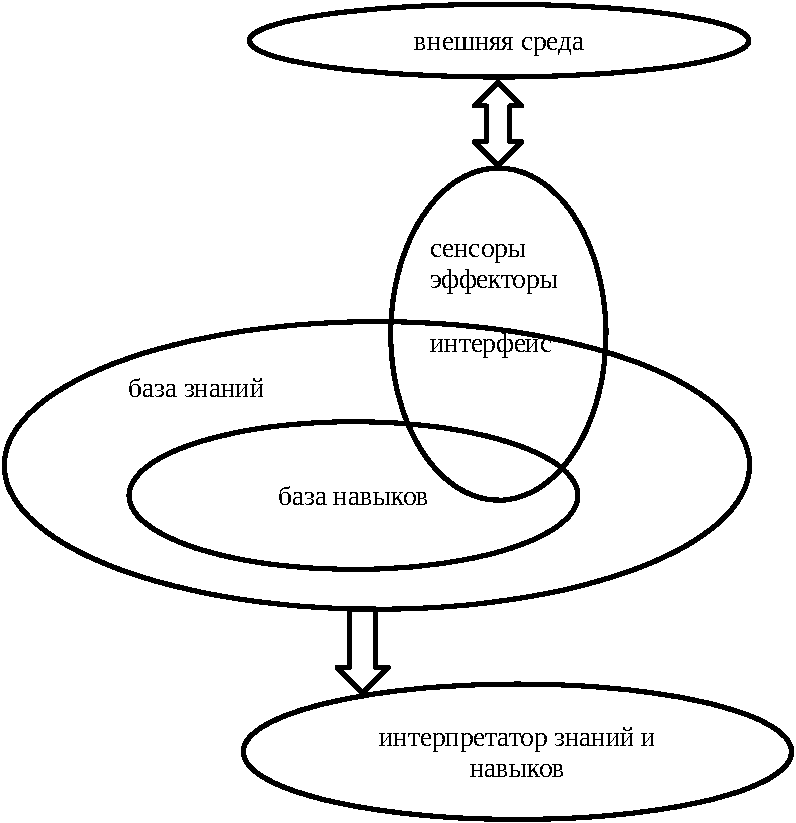
\includegraphics[width=0.5\linewidth]{figures/arch.pdf}\\}

\bigskip
\scnendstruct \scnendcurrentsectioncomment

\end{SCn}